\documentclass[11pt, oneside]{article}   	% use "amsart" instead of "article" for AMSLaTeX format
\usepackage{geometry}                		% See geometry.pdf to learn the layout options. There are lots.
\geometry{letterpaper}                   		% ... or a4paper or a5paper or ... 
%\geometry{landscape}                		% Activate for for rotated page geometry
%\usepackage[parfill]{parskip}    		% Activate to begin paragraphs with an empty line rather than an indent
\usepackage{graphicx}				% Use pdf, png, jpg, or eps� with pdflatex; use eps in DVI mode
								% TeX will automatically convert eps --> pdf in pdflatex		
\usepackage{amssymb}
\usepackage{amsmath}
\usepackage{parskip}
\usepackage{color}
\usepackage{hyperref}

\title{Laurent series}
%\author{The Author}
%\section{}
%\subsection*{}
\date{}							% Activate to display a given date or no date

\graphicspath{{/Users/telliott_admin/Dropbox/Tex/png/}}
% \begin{center} 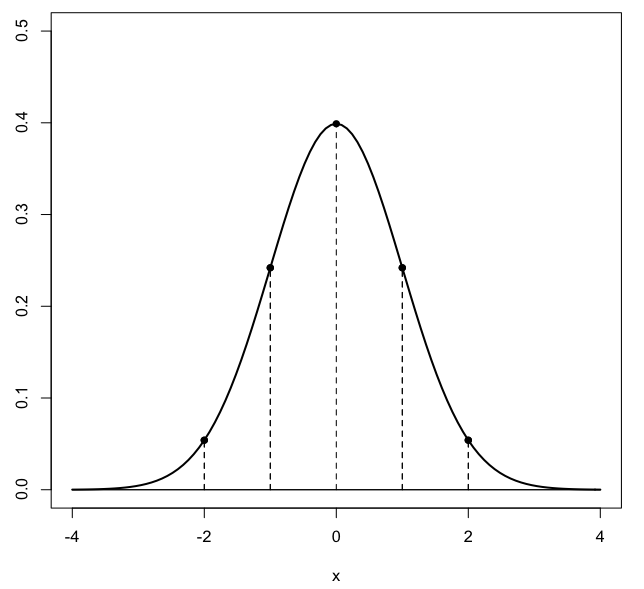
\includegraphics [scale=0.4] {gauss3.png} \end{center}
\begin{document}
\maketitle
\Large
The Laurent series of a complex function $f(z)$ is a representation of that function as a power series which includes terms of negative degree (wikipedia).

For a function expanded about a point $z_0$ the series is
\[ f(z) = \sum_{n=-\infty}^{\infty} a_n(z-z_0)^n \]
To determine a particular coefficient $a_k$, multiply both sides of the above expression by $1/(z-z_0)^{k+1}$ and integrate around a closed path
\[ \oint \frac{f(z)}{(z-z_0)^{k+1}} \ dz = \sum_{n=-\infty}^{\infty} \oint a_n \frac{(z-z_0)^n}{(z-z_0)^{k+1}} \ dz \]
Recall that all the $a_n$ are constants and can come outside the integrals.  
\[ = \sum_{n=-\infty}^{\infty}  a_n \oint \frac{(z-z_0)^n}{(z-z_0)^{k+1}} \ dz \]
Only one term in the infinite series on the right is non-zero.  That is the term where $n=k$
\[ = a_n \oint \frac{1}{(z-z_0)} \ dz \]
We know this one, it is:
\[ = a_n \ 2 \pi i \]
(If you doubt this, substitute $w = z - z_0$, so $dw = dz$ and we have
\[ \oint \frac{dw}{w}  = 2 \pi i \]
Thus 
\[ 2 \pi i \ a_n = \ \oint \frac{f(z)}{(z-z_0)^{n+1}} \ dz \]
\[ 2 \pi i \ a_{-1} = \ \oint \frac{f(z)}{z-z_0} \ dz \]



\end{document}  